\documentclass[11pt,a4paper]{article}

\usepackage[utf8]{inputenc}
\usepackage[magyar]{babel}
\usepackage[T1]{fontenc}

\usepackage{makecell}
\usepackage{graphicx}

\newcommand{\q}[1]{„#1''} % Redefine quotations

\title{Blockchain - a \textit{block chain}}
\author{Pál Balázs}
\date{2018. december 17.}

\begin{document}

\maketitle

\section{Bevezetés}
A \textit{blockchain} techonlógáját, annak alapvető felépítése miatt a kriptográfia és a peer-to-peer hálózatok témaköréhez kapcsolódóan említhetjük. A blockchain szorosan összefonódik a kriptovaluták fogalmával, hisz 2008-ban a Satoshi Nakamoto néven futó, máig ismeretlen feltalálója/feltalálói a Bitcoin valutájához használatos \q{tranzakciós főkönyv} szerepét betöltendő fejlesztették ki.

\section{Motiváció}
Ahhoz, hogy a blockchain létjogosultságát és motivációját megérthessük, előbb meg kell ismerkednünk azzal, hogy a mai pénzügyi világban a \q{pénz} dinamikája nagy vonalakban, leegyszerűsítve hogy is működik. A Bitcoin világban elfoglalt helyzetének és az utolsó fejezetben található kitekintésben foglaltak megértéséhez a \q{pénznek} a jelentését kell legelőször tisztáznunk.
\\ \\
Azt, hogy pontosan mi is ez, azt több szükséges kondíció egyidejű megléte definiálja. Pénz minden olyan meghatározott értékkel bíró tárgy, amely:

\begin{enumerate}
    \item Értékmérő, tehát a termékek árai, a jövedelmek és az adósságok mértéke, mind a pénzen keresztül, a \q{pénz által mérve} határozódik meg.
    \item Forgalmi és fizetési eszköz, azaz közvetítő szerepet tölt be a gazdasági ügyletek\footnote{gazdasági ügyletek: Két fél között zajló tranzakció: pl. áruk forgalmánál létrejövő tranzakciók} során. Egy ilyen ügylet szereplői azért fogadják el a pénzt ilyen közvetítő eszközként, mert bármilyen másik ügyletben is képes ezt a szerepét betölteni.
    \item Értékálló, tehát felhalmozásra, tartalékolásra alkalmas, értéke stabil és nem csökkenő. Mindkét előző funkcióhoz szükséges, hogy a pénz az egymást követő ügyletekben változatlan bizalmat kapjon a résztvevőktől, azaz a pénz megőrizze az értékét.
    \item A fenti kondíciók megléte mellett a piac által is elfogadott pénzként.
\end{enumerate}

\noindent A modern banki rendszer - amikben tehát a fent tárgyalt \q{pénz} a közvetítő - ma még nem teljesen globális. Egy tranzakció egy pénzügyi zónán belül viszonylag gyors, de pénzügyi zónák között (pl. Európa és Észak-Amerika) még nagyon lassú és költséges. Pl. Európán belüli banki utalásnál (2018-tól már nem csak euróövezeten belül) szinte perceken belül és többletköltségek nélkül teljesül egy tranzakció, de pl. az USA-ba utalva ez akár napokba is telhet. Egy leegyszerűsített képen megérthetjük, hogy ez miért is van így. \\
Minden olyan ügyletet, ami - legtöbb esetben (az extravagáns helyzeteket nem figyelembe véve) - egy bankon keresztül, vagy bankok között történik, azt a közvetítő/felügyelő szerv köteles feljegyezni egy ún. főkönyvbe. Ez a főkönyv arra szolgál, hogy időrendben követhető legyen minden pénzügyi/gazdasági művelet. Ebbe feljegyzésre kerülnek pl. banki átutalások, kártyával történő fizetések, számlafizetések, bérek kifizetései, stb., tehát minden pénz mozgása. \\
Hogy ezek többsége megvalósítható legyen, értelemszerűen az embernek egy bankban meg kell bíznia és a bankkal szerződést kell kötnie, hogy ott számlát nyithasson, amivel aztán a fent felsorolt és azokhoz hasonló tranzakciókat végezhessen. Amikor egy ember számlát nyit egy bankban és arra pénz utal - előre meghatározott feltételek mellett -, az a gyermeki fantáziával ellentétben nem ül aranyrögök formájában egy széfben, hanem a bank azt a pénzt befekteti. Pl. leggyakrabban más ügyfeleknek fizet éves járadékot a befektetett pénzük után, vagy épp kifizet egy olyan ügyfelet, aki a bankból a pénzét ki szeretné venni. Ehhez a banknak szüksége van valami olyan megfelelő alapra, amiből krízis esetén is képes az ügyfeleknek fizetni. Ezeket általában ún. likvid eszközök\footnote{likvid eszköz: Olyan pénzügyi eszköz, amelyet könnyedén, különösebb tranzakciós költségek nélkül pénzzé lehet tenni} formájában halmozza fel a bank. Mikor egy banknak kezdenek elfogyni az ilyen eszközei, akkor más bankkal köt valamilyen szerződést - természetesen ugyanolyan bizalmi alapon, mint a fent leírt számlanyitás esetében -, hogy likvid eszközökhöz jusson. Az ilyen szerződések megkötése általában a tőzsdén történik a bankok brókerei által. Ilyen likvid eszközök folyamatos ide-oda áramlása biztosítja, hogy a bankok az adott országban folyamatosan ki tudják elégíteni az ügyfelek igényeit, miközben befektetésekből és tranzakciós illetékekből ők maguk is pénzhez jutnak. \\
Ma a tranzakciók egy adott pénzügyi zónában azért lehetnek gyorsak és olcsóak, mert a zónán belül van egy egységes, centralizált szerv, aki felügyeli a gazdaságot, mindenhol azonos és azonosan érvényes szabályok mellett. A legtöbb lépés mára már gépiesített, ami pont azért lehetséges, mert egy egységes, zárt zónán belül nincs szükség különböző szabályokkal működő felek közötti manuális szerződéskötésre és megállapodásra, hisz nincsenek ilyenek.
\\ \\
Ellenben Európa és Észak-Amerika felett nincs egy egységes rendszer, a két zóna eltérő szabályokkal, eltérő dinamikával rendelkezik. A kettő között történő pénzügyi eszközök áramlásához szükség van emberi beavatkozásra, szerződések megkötésére, stb. Ehhez megint szükség van arra is, hogy a két fél megbízzon egymásban, tehát abban, hogy a szerződés másikra eső fele is teljesülni fog és hogy egyikük sem fog veszteséget elszenvedni a másik fél miatt.
\\ \\
A Bitcoinhoz létrehozott még - külön írt - \q{block chain} nevű rendszer a 2008-as gazdasági világválság kirobbanása idején jött létre. Egészen pontosan a \q{bitcoin.org} domaint 2008. augusztus 18-án regisztrálták, a rajta szereplő \textit{Bitcoin: A Peer-to-Peer Electronic Cash System} című, egy \textit{Satoshi Nakamoto} nevű szerzőt feltüntető dokumentumra mutató linket pedig 2008. október 31-én tették közzé egy kriptográfiai témájú levelezőlistán. Maga a Bitcoin végül 2009. január 9-én lett egy open-source szoftver (a Bitcoin Core) formájában megjelentetve. \\
Maga a 2008-as világválság a fenti, most csak leegyszerűsített formában vázolt rendszer egy láncszerűen terjedő krízise miatt következett be. Ami történt, az pont a többször is szándékosan hangsúlyozott bizalmi tényező megszűnésének tudható be. A bankok elvesztették egymásban és a centrális felügyelő szervben a bizalmat, majd miután hirtelen így láncszerűen szinte egy bank se tudta teljesíteni az ügyfelek felé ígért és szerződésben kötött kötelezettségeit, az emberek is elvesztették a bizalmukat a bankokban. \\
Ebben a kialakult káoszban, pont a számára legszerencsésebb időpontban jött létre a Bitcoin. A blockchain első block-ját (ami emiatt a \textit{genesis block} nevet kapta és amikről a továbbiakban részletesebben szó lesz, hogy pontosan micsodák) 2009. január 3-án bányászta ki megalkotója, a Satoshi Nakatomo névvel illetett entitás. A block-ba a - minden block-ban megtalálható - időpecsét mellett az alábbi üzenet volt beillesztve: \textit{\q{The Times 03/Jan/2009 Chancellor on brink of second bailout for banks.}} Ez tulajdonképpen az aznapi londoni The Times főcíme volt, amit manapság úgy interpretálnak, mint egy afféle kommentár és piszkálódás a bankok felé, kritizálva azok rendszerét, ami végül a világválsághoz vezteztett.

\section{Felépítés és működés - Az ötlet és ami mögötte van}
A blockchain valódi célja az volt, hogy egy olyan elektronikus pénzügyi rendszert hozzon létre, amiben teljes mértékben ki tudjuk zárni a bizalmi faktort. Másrészt a blockchain egy olyan elektronikus főkönyvként szeretne szolgálni, amihez nem szükséges egy centralizált felügyelet, és amit meghamisítani, vagy megbabrálni lehetetlen. Ehhez a peer-to-peer hálózatokat és a kriptográfiát hívta Satoshi Nakamoto segítségül.\\
Maga az ötlet nem teljesen új. 1991-1992 körül voltak már kutatások arról, hogy hogyan lehet a kriptográfia segítségével egy block-hálózatot felépíteni, amely segítségével egy dokumentumban található időpecsétek buherálása lehetetlenné válik. Ezt a gondolatot fejlesztette/fejlesztették tovább a Bitcoinhez létrehozott blockchain esetében, csak itt nem szimplán dokumentumok időpecsétjének, hanem tranzakciók adatainak megváltoztathatatlanná tétele volt a cél. \\
A következőkben előbb a blockchain vázlatos felépítéséről lesz szó, az egyes részleteket utána tárgyalom.

\subsection{A blockchain}
Egy nagyon könnyen megérthető példával lehet a legjobban szemléltetni, hogy hogyan működik a blockchain rendszere és hogy mely része minek feleltethető meg a való életben. \\
Tegyük fel, hogy van egy főkönyv, amiben egy társaság folyamatosan vezeti az egymás közötti tranzakciókat. Ez a következőképp fest:

\begin{center}
\begin{tabular}{c|c}
Sorszám & Bejegyzés \\
\hline \hline
1. & Anna adott Tominak 100 forintot \\
\hline
2. & Peti adott Annának 150 forintot \\
\hline
3. & Jani adott Lacinak 70 forintot \\ 
\hline
\vdots & \vdots
\end{tabular}
\end{center}

\noindent Ez nem a legbiztonságosabb, mert bárki meg tudna változtatni bármelyik bejegyzést észrevétlenül. Az első ötlet ennek kiküszöbölésére a Hash függvény használata, aminek a tulajdonsága, hogy bármilyen hosszú szöveget képes mindig ugyanolyan hosszú, a függvény bemenete által meghatározott karakterek sorozatára (\textit{string}-é) transzformálni, visszafejteni azonban szinte lehetetlen. Ezt a kapott karakterláncot hívjuk hash kódnak. Két, bitre pontosan megegyező szöveg hash kódja megegyezik, azonban már a legapróbb változtatás is az eredeti szövegben hatalmas különbséget okoz a kapott hash kódok között. Próbáljunk meg most minden tranzakciót ilyen hash kód formájában tárolni:

\begin{center}
\begin{tabular}{c|c}
Bejegyzés & Hash kód \\
\hline \hline
Anna adott Tominak 100 forintot & \scriptsize{8ECA4C4B91C975A26F9F8EE17002E8EF3C68395A} \\
\hline
Peti adott Annának 150 forintot & \scriptsize{4819829BB346A970BDBC793BD8AC18C443919E88} \\
\hline
Jani adott Lacinak 70 forintot & \scriptsize{B109055B514F958A8F206ACC8F86B2FFAF2C4D9A} \\ 
\hline
\vdots & \vdots
\end{tabular}
\end{center}

\noindent Sajnos ez a megoldás se jó még, hisz ha valaki más is ismeri a Hash függvényt, akkor könnyen megváltoztathatja a bejegyzést és a hozzá tartozó hash kódot. Következő ötletünk, hogy minden bejegyzés végére illesszük oda az előző bejegyzés hash kódját, és az így kapott karakterláncot fordítsuk le a Hash függvénnyel. Ez így fog kinézni ebben az esetben:

\begin{center}
\begin{tabular}{c|c}
Bejegyzés & Hash kód \\
\hline \hline
Anna adott Tominak 100 forintot & \scriptsize{8ECA4C4B91C975A26F9F8EE17002E8EF3C68395A} \\
\hline
\makecell{Peti adott Annának 150 forintot \\ \scriptsize{8ECA4C4B91C975A26F9F8EE17002E8EF3C68395A}} & \scriptsize{545304E7A452E56FA9472F36D52EDA77EF7687F1} \\
\hline
\makecell{Jani adott Lacinak 70 forintot \\ \scriptsize{545304E7A452E56FA9472F36D52EDA77EF7687F1}} & \scriptsize{9A74836ED4F293116C4C3B03925365BA2FDEC40C} \\ 
\hline
\vdots & \vdots
\end{tabular}
\end{center}

\noindent Így minden új cella értéke függeni fog az előtte levőtől. Ha egyet valaki meg akar változtatni, az összes létező utána következőt meg kell változtatnia. Hogy még tovább bonyolítsuk az egészet, bevezetünk egy úgynevezett \q{Nonce}-ot, aminek a szerepe a következő:

\begin{center}
\begin{tabular}{c|c}
Bejegyzés & Hash kód \\
\hline \hline
Anna adott Tominak 100 forintot 948 & \scriptsize{52126ba80c8fa3bda71536fffb4ab01bb6590800} \\
\hline
\makecell{Peti adott Annának 150 forintot 169 \\ \scriptsize{52126ba80c8fa3bda71536fffb4ab01bb6590800}} & \scriptsize{3cf9d7c602e473b2008d5cb00b3c3c21adc11b00} \\
\hline
\makecell{Jani adott Lacinak 70 forintot 148 \\ \scriptsize{3cf9d7c602e473b2008d5cb00b3c3c21adc11b00}} & \scriptsize{dc694b79d833f37029e250b62ac0b94970a73e00} \\ 
\hline
\vdots & \vdots
\end{tabular}
\end{center}

\noindent Az eredeti bejegyzés szövegéhez hozzáfűzött párjegyű szám - ez a Nonce - azt eredményezi, hogy a teljes bejegyzés output hash kódjának utolsó két számjegye 00 lesz. Ahhoz tehát, hogy minden bejegyzést megváltoztassunk, ahhoz minden egyes bejegyzéshez tartozó Nonce-ot is ki kell számítanunk.
\\ \\
Tegyük fel, hogy kezd nagyon sok bejegyzés lenni egy idő után ebben a főkönyvünkben. Egy adott darabszámnál azt mondjuk, hogy elég, az eddigi tranzakciókról szóló listát lezárjuk és a tartalmát rámásoljuk egy egyoldalas dokumentumra. Valakivel ellenőrizzük, hogy minden rendben van a tranzakciókkal, majd a dokumentumot lemásoljuk és szétszórjuk rengeteg számítógép között a világban. Ezek a számítógépeket - amiket egyesével \textit{node} néven hívunk - innentől birtokában lesznek ennek a rengeteg tranzakciót tartalmazó főkönyvnek. Ezt az egyoldalas összesítést hívjuk egy \textit{block}-nak, ezek láncolatát pedig \textit{blockchain}-nek. \\
Minden egyes node-nak van egy másolata az aktuális blockchain-ről, ami 10 perces etaponként, minden számítógépen egyszerre frissül. Ha egy új block keletkezik - miután az is elért egy adott tranzakciós limitet - akkor történik az a folyamat, amit a kriptovalutáknál történő alkalmazása miatt \q{mining}-nak, vagy magyarul \q{bányászás}-nak hívunk. Ez több részből áll: Első feladat, hogy a \q{bányász node}-ok leellenőrizzék az adott block-ban szereplő tranzakciók validitását. Tényleg nem történt-e a bejegyzések illetéktelen módosítása? Ha mindent rendben találnak, akkor következik a következő lépés: Az ezen block-ot közvetlenül megelőző block adatait felhasználva le kell generáljanak egy speciálisan megadott hash kódot, amit aztán hozzáillesztve az új block-hoz, láncszerűen összekapcsolhatják a kettőt. A kód generálása az előző block adataihoz hozzáfűzött nonce megtalálásával történik, a cél pedig hogy a kapott hash kód egy konkrét, a blockchain által meghatározott intervallumban legyen. Maga a bányászás lényegi része ez a folyamat, ez amihez nagy számítási teljesítmény szükséges. Amikor egy bányász node megtalálja a megfelelő nonce-t és a hozzá tartozó hash kódot, akkor ez a kód és nonce, mint egy pecsét, beleíródik a következő block adatai közé, és a block csatlakozik a blockchainhez. Ez a Bitcoin esetében a konkrét gyakorlatban azt jelenti, hogy egy olyan hash kódot kell megtalálni, ami megadott darabszámú 0-val kezdődik. A megfejtő ezután Bitcoinokat kap jutalomként a blockchaintől, valamint a \q{megfejtett} block-ban található tranzakciók \q{kezelési költségét} is megkapja. \\
Ezután az egész kezdődik elölről, megtelik egy újabb block, megtörténik a validációja, \q{kibányászása}, majd hozzáfűződik a blockchain végére. \\

\subsection{A tranzakciók és a blokkok felépítése}
Fent egy leegyszerűsített verziójáról volt szó a blockchainnek, ami csupán a valódi képnek csupán a keretét mutatta be. Belső felépítése valójában jóval részletesebb, erről lesz szó a továbbiakban.
\\ \\
A node-ok egymással egy decentralizált, ún. peer-to-peer hálózaton keresztül kommunikálnak. Ez azt jelenti, hogy minden node csak néhány tetszőleges node-al áll összeköttetésben, mindenféle középpont megléte nélkül. Ezen a hálózaton keresztül biztosítja a blockchain, hogy minden node-on 10 percenként frissítse magát, valamint több fontos kommunikáció is történik. \\
Az egyik ilyen a tranzakciók létrejötte. Míg a valódi pénzügyi rendszerekben a tranzakciók általában titkosítottak, addig a blockchain esetén azok teljesen publikusak, létrejöttük pillanatában \q{belekiabálódnak} a hálózatba. Ezek a tranzakciók azonban csak akkor íródhatnak bele egy új blokkba, ha azt a node-ok egy afféle szavazással validálják. Erre két ok miatt van szükség:

\begin{enumerate}
    \item Nincs egy központi felügyeleti centrum, ami képes minden tranzakciót ellenőrizni
    \item Egy adott digitális pénzmennyiséget csupán egyszer szabad, hogy a tulajdonosa elköltsön
\end{enumerate}

\noindent Azt biztosítandó, hogy egy tulajdonos csak egyszer költhessen el valamekkora mennyiségű Bitcoint, ahhoz a róla szóló tranzakciót ellenőrizni kell, és felvinni a rendszerbe. Ha nincs központi ellenőrző ún. \q{mint}, akkor ehelyett más megoldást kell találni. A blockchain azt a megoldást válaszotta, hogy a Bitcoin tranzakciókat kényszerűen publikussá tette, amik láncszerűen, időrendben hitelesítik egymást. Ezek block-ba tömörödnek, ezeket pedig a node-ok együttesen ellenőrzik és validálják majd a mining elején. Ez a metódus volt felvázolva a fenti egyszerű példában is. A gyakorlatban ez valamivel bonyolultabban működik. Ahhoz, hogy tranzakciók folyhassanak két node között, a node-nak rendelkeznie kell egy \textit{wallet}-el, tehát egy \q{pénztárcával}, ami a bankszámla szerepét tölti be a kriptovaluták világában. Ez a wallet igazából egy public-private key párosból áll, ahol a public key a wallet-et (tehát tulajdonképpen a bankszámlaszámot) jelöli. Amikor két wallet között megtörténik egy tranzakció, akkor a következők történnek:

\begin{enumerate}
    \item Az első bejegyzés egy block-ban az ún. \q{coinbase}, ami az előző block kibányászatáért járó jutalomról szóló tranzakciót tartalmazza, valamint összekapcsolja az aktuális block-ot az előző block-al.
    \item Mikor megtörténik az első ezt követő tranzakció, abban elsődlegesen két fontos dolog fog szerepelni. Első adat az előző tranzakció output-jára mutató hash (jelen esetben ez a coinbase), második pedig egy scriptSig névre hallgató azonosító. Ez a tranzakcióban a fogadó fél wallet-jének public key-jét, valamint a küldő private és public key-ből generált aláírását fogja tartalmazni.
    \item Ez ezután felvételre kerül az aktuális block-ba, a coinbase után, és kapni fog egy bekerülésről szóló időpecsétet.
\end{enumerate}

\begin{center}
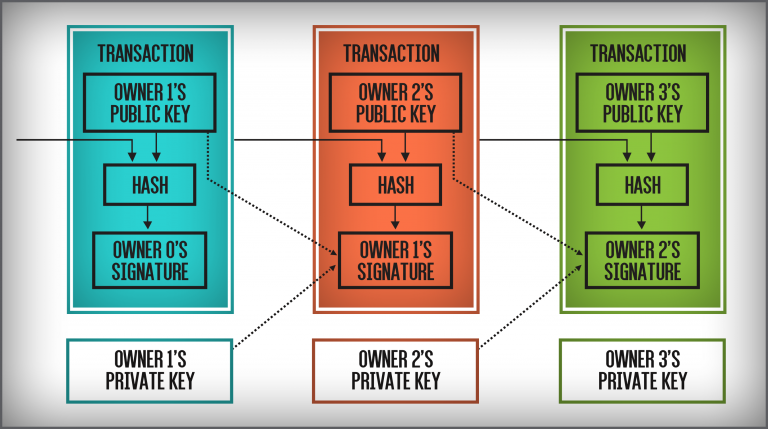
\includegraphics[width=0.75\textwidth]{transactions.png}
\end{center}

\noindent A tranzakciók egymás után gyűlnek fel az aktuális blokkban, majd 10 perc után a rendszer frissül. Ezen 10 perc alatt felhalmozódott tranzakció költségeiből, a block header-jébe az ún. \q{Merkele tree} alapján egy \textit{top hash}/\textit{root hash} helyeződik el az előző block-ból származó hash és a hozzá kapcsolódó nonce mellett. Hogy ez átlagosan mindig 10 perc legyen, a rendszer folyamatosan úgy állítja be a szükséges megoldandó matematikai probléma nehézségét, hogy tényleg kb. 10 percenként bányászódjon ki egy block, és azonnal rá lehessen térni a következőre.
\\ \\
A számítási teljesítmény folyamatos növekedésével is számoltak az alkotók, hisz időben a block-ok bányászatának nehézsége egy adott faktor szerint konstans módon növekedik. Emellett a kibányászásért járó Bitcoin jutalom folyamatosan csökken.

\subsection{51\% attack}
A blockchain felépítéséből származóan van egy, már Satoshi Nakamoto cikkében is tárgyalt gyengepont, amire a blockchain nem tud megoldást kínálni. A blockchainben természetes módon, vagy szándékos támadás folytán is létrejöhetnek afféle \textit{elégazások}. Ez általában akkor fordul elő, ha két node azonos időben bányászik ki egy block-ot, de olyan esetben is kialakulhat, amikor egy támadó megpróbálja visszafejteni - az elején ismertetett, egyszerű példában leírt módon - a block-okat, és létrehozni egy saját ágat, ezzel teljes uralma alá hajtania a rendszert. A blockchain képes arra, hogy ilyen esetben az egyes ágakat valamilyen relevancia alapján egy algoritmus szerint pontozza, és így mindig egy konkrét ágat előnyben részesítsen a többivel szemben. Ilyenkor A kisebb pontszámot kapott ág \textit{orphan block}-á, magyarul \textit{árva block}-á válik, a lánc ott nem folytatódhat, hanem a blockchain által választott ágon kell folytatódjon. Az árva block-okban levő adatok a fő lánc egy új block-jába íródnak ilyenkor.
\\ \\
A blockchain fentebb is tárgyalt legfőbb újítása, hogy az ún. \textit{double-spending}-et, tehát ugyanazon mennyiségű valuta kétszeri elköltését a tranzakciók validálásának láncával lehetetlenné teszi. Ez egészen addig igaz is, míg valaki nem szerez kontrollt a tranzakciók validálása felett. Elméletben ha valaki a rendszer számítási teljesítményének több, mint 50\%-ával rendelkezik, képessé válik erre. \\
A folyamat viszonylag egyszerű. A támadó a fő blockchainről elágazva, egy \textit{privát} láncot (\textit{stealthchain}) kezd el folytatni. Az ebben bányászott block-okat azonban nem osztja meg a többi node-al, hanem megtartja magának. Itt kezdődik a probléma. Tegyük fel, hogy a támadó Bitcoint költ, amely tranzakciót a főláncon bejegyzi, de a saját, privát láncában nem. Ha a támadó több, mint a teljes számítási teljesítmény 50\%-áz uralja, képes \q{leelőzni} a publikus, fő blockchain-t, és hosszabb láncot létrehozni a saját ágán, mint a publikus. 

\begin{center}
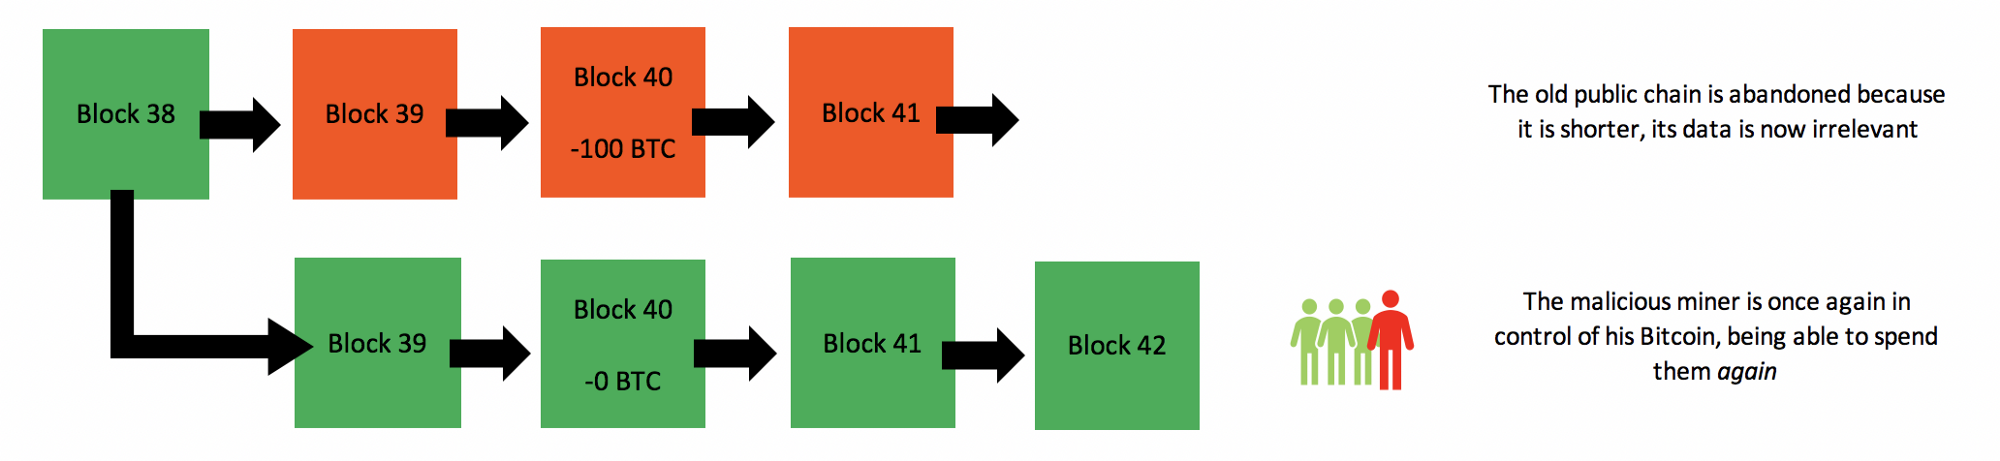
\includegraphics[width=\textwidth]{stealthchain.png}
\end{center}

\noindent Ha a támadó ekkor megosztja a saját stealthchain-ének adatait a többi node-al, akkor a blockchain azt fogja látni, hogy az ő ága \textit{hosszabb} és emiatt értékesebb, mint az eddig publikusnak számító ág. Ilyenkor a támadó saját ága válik \q{aktívvá}. Ekkor minden, a másik ágon létrejött tranzakció semmissé válik és a saját - eddig - privát ágán bejegyzett tranzakciók válnak validálttá.

\section{Megoldást kínál a létrejöttét motiváló problémára? - Kitekintés (APA CIKKÉNEK VÉGE)}
A bitcoin pénzzé válása előtt álló probléma, hogy sikeresebb pénzügyi eszközként, mint pénzként, előbbi sikerének következményei gátolják az utóbbit. A bitcoin a jelenleg használt pénzzel szemben, így minden más dologgal szemben is amit pénzben mérünk vagy fejezünk ki, hektikusan változtatja az értékét. Árfolyama hihetetlenül jelentős változékonyságot mutat. 
\\ \\
Amíg ez így van, értékmérőként használhatatlan. Az árakat nem lehet bitcoinban megadni, hiába fogadják el sok helyen fizetésre, az árakat döntően dollárban, euróban stb. fejezik ki az eladók. Bitcoinban hitelt felvenni képtelenség.  Az árfolyam emelkedése komolyan veszélyezteti a bitcoin tranzakciós használatát. A tranzakciós költségek bitcoinban adottak, ezért a bitcoin árfolyamának emelkedésével a tranzakciók is jelentősen drágultak. Azaz a bitcoinban végrehajtott fizetések elveszthetik kezdeti költségelőnyüket az alternatív fizetési módokkal szemben. Természetesen, a bitcoint egyetlen állam sem ismeri el hivatalos fizetőeszköznek, azaz adót sem lehet vele fizetni.
\\ \\
Monetáris politikai szempontból elsősorban az árstabilitás biztosítása a fontos. Akárcsak az első világháborúig haasználatos aranypénzrendszer, a bitcoin mögött álló rendszer sem képes a mai modern gazdaság stabilitási és növekedési igényeinek megfelelő árstabilitást, a tartósan alacsony inflációt biztosítani. Ezért a bitcoin pénzzé válásához a mögöttes monetáris paramétereket és szabályokat is ennek megfelelően át kellene szabni.
\\ \\
Azt világosan kell látni, hogy a bitcoin valós, fundamentális értéke abból származhat, ha pénzként funkcionál. Ha nem képes erre, akkor pusztán egy digitális játékszer marad, amelynek árát csak a túlfűtött spekulációs haszonszerzés reménye fújja fel. 

\end{document}
